\documentclass[11pt]{article}
\usepackage[utf8]{inputenc}
\usepackage[T1]{fontenc}
\usepackage{graphicx}
\usepackage{longtable}
\usepackage{float}
\usepackage{wrapfig}
\usepackage{soul}
\usepackage{amssymb}
\usepackage{hyperref}
\usepackage[spanish]{babel}
\usepackage{bookman}
\usepackage[left=3cm,top=3cm,right=2cm,bottom=1cm,head=1.5cm,includefoot]{geometry}
\usepackage{listings}
\usepackage{multirow}
\usepackage{amssymb}
\usepackage{fancyhdr}
\usepackage{comment}
\usepackage{color}
\usepackage{multicol}
\usepackage[table]{xcolor}
\usepackage{ulem}

\title{informe}
\author{}

\begin{document}

% ---------------------- Encabezado y pie de página -----------------------

% Encabezado: sección a la derecha.
% Pie de página: número de página a la derecha.

\pagestyle{fancy}
\renewcommand{\sectionmark}[1]{\markboth{}{\thesection\ \ #1}}
\lhead{}
\chead{}
\rhead{\rightmark}
\lfoot{ $2^{o}$ Cuatrimestre 2011, Trabajo práctico $N^{o}2$, Grupo 1: 88.581,}
\cfoot{}
\rfoot{ 88062, 88.246 - p\'agina \thepage}


% Hago que las páginas se comiencen a contar a partir de aquí.
\setcounter{page}{1}

% Índice
\tableofcontents
\newpage


\section{Enunciado}

\begin{center}
% Orden del trim = izq abajo derecha arriba
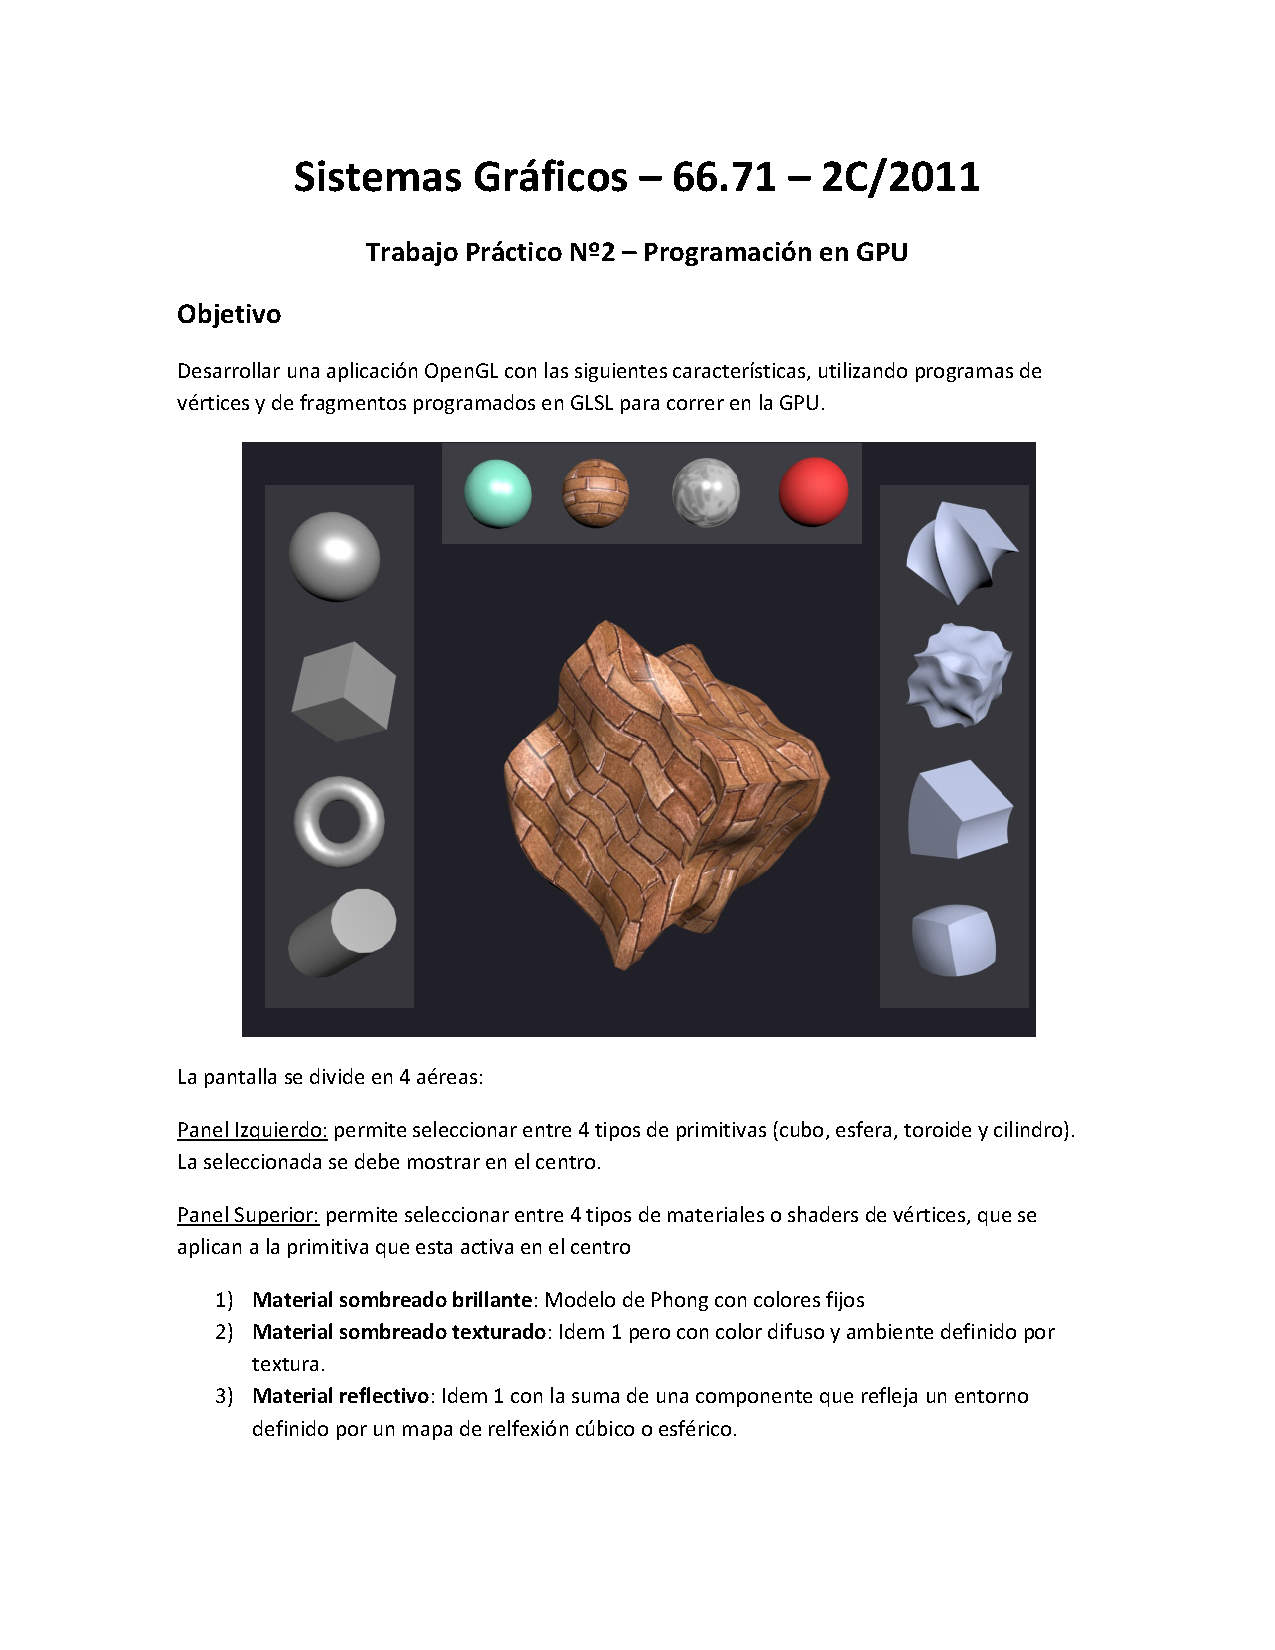
\includegraphics[trim = 25mm 30mm 10mm 35mm, clip,height=0.93\textheight,width=1.04\textwidth]{tp2-c2-2011.pdf}
\includegraphics[trim = 25mm 20mm 10mm 25mm, clip,height=0.95\textheight,width=1.04\textwidth,page={2}]{tp2-c2-2011.pdf}
\includegraphics[trim = 25mm 20mm 10mm 25mm, clip,height=0.95\textheight,width=1.04\textwidth,page={3}]{tp2-c2-2011.pdf}
\end{center}

\newpage


\section{Consideraciones de Dise\~no}
Para realizar el presente trabajo pr\'actico se utiliz\'o el lenguaje de programaci\'on GLSL dado que el mismo permite programar la GPU 
de la tarjeta de video para realizar c\'alculos complejos con una mejor performance y precisi\'on.
  Para realizarlo, se tomaron en cuenta las siguientes consideraciones de dise\~no:
\begin{itemize} 
 \item Se debi\'o utilizar la versi\'on 1.2 de GLSL dado que es la soportada por las tarjetas gr\'aficas de las notebooks de la mayor\'ia de 
los integrantes del grupo.
 \item Se decidi\'o agregar la funcionalidad de girar la primitiva seleccionada con respecto a los tres ejes (x,y,z) en ambos sentidos, utilizando teclas espec\'ificas del 
teclado (Ver {\bf Controles del teclado} para mayor informaci\'on).
 \item Se agreg\'o el cono como uno de los tipos de primitivas disponibles para seleccionar.
 \item Para el mapeo de texturas en la superficie reflexiva se utiliza un mapa c\'ubico.
 \item Se supone que la reflecci\'on obtenida de la superficie brillante es la m\'axima.
 \item La componente ambiental de las luces puntuales es una luz de color negro.
 \item Se utiliz\'o la librer\'ia Il (devil) para cargar las texturas en formato .png, que luego son mapeadas en el mapa c\'ubico utilizado para el 
material reflectivo.
\end{itemize}


\subsection{Estructura de la aplicaci\'on}
Para desarrollar la aplicaci\'on se utiliz\'o el lenguaje C++, que permite la programaci\'on orientada a objetos con el encapsulamiento de clases. 
Dentro de las principales, se encuentra la clase Mundo; que representa el mundo del trabajo pr\'actico en el cual se suscriben los eventos de OpenGL. 
Contiene los men\'ues de los distintos paneles y la primitiva seleccionada, y responde a las peticiones del usuario. \\\\
 Se utiliz\'o el patr\'on Command para el manejo de teclas, movimiento del mouse y el click del mouse en los elementos de los men\'ues. 
Entre estos \'ultimos, se encuentran los comandos cambiar textura, cambiar color, cambiar forma, etc.\\\\
 Existen shaders de vertices, que realizan principalmente las transformaciones de las deformaciones, shaders de iluminaci\'on (basando los c\'alculos en el modelo de Phong) y
shaders de fragmentos que combinan la iluminaci\'on con la textura y el material de la primitiva seleccionada. 

\newpage

\section{Compilaci\'on}
  Para compilar la aplicaci\'on bajo entorno Linux se provee un archivo makefile.
  Para utilizar el mismo, debe tenerse instalada la herramienta cmake. Para instalarla, por ejemplo, en una distribuci\'on Ubuntu se deben 
realizar los siguientes pasos: \\
1) sudo apt-get install cmake \\
2) Ingresar la contrase\~na de root del usuario. \\
3) Aceptar la descarga e instalaci\'on de los paquetes necesarios. \\ 

Teniendo ya instalada la herramienta, posicionados en el directorio donde se encuentra el trabajo pr\'actico es necesario crear un directorio build
de la siguiente forma: \\
mkdir build \\
cd build \\
cmake .. \\
make \\

Una vez realizados estos pasos, se dispondr\'a del ejecutable de nombre tp2.

\section{Ejecuci\'on}

Para ejecutar la aplicacio\'n bajo un entorno Linux se deben realizar los siguientes pasos: \\
1)Posicionarse en el directorio build creado anteriormente. \\
2)Ejecutar: \\
./tp2 

\newpage
\section{Controles de teclado}

La aplicaci\'on permite realizar las siguientes acciones utilizando las teclas detalladas a continuaci\'on: \\


    \begin{tabular}{|| l | l ||}
      \hline
      \begin{large}Tecla\end{large} & 
	\begin{large}Acci\'{o}n \end{large} \\
          \hline
x & Rotar la primitiva seleccionada con respecto al eje x en el sentido positivo. \\
X & Rotar la primitiva seleccionada con respecto al eje x en el sentido negativo. \\
y & Rotar la primitiva seleccionada con respecto al eje y en el sentido positivo. \\
Y & Rotar la primitiva seleccionada con respecto al eje y en el sentido negativo. \\
z & Rotar la primitiva seleccionada con respecto al eje z en el sentido positivo. \\
Z & Rotar la primitiva seleccionada con respecto al eje z en el sentido negativo.  \\
q & Salir de la aplicaci\'on.  \\
r & Resetear las transformaciones y/o deformaciones aplicadas a la primitiva seleccionada.  \\
c & Captura/libera el movimiento del mouse para rotar la primitiva seleccionada.  \\
m & Muestra/esconde los menues.  \\
1 & Encender/apagar la fuente de luz 1.  \\
2 & Encender/apagar la fuente de luz 2.  \\

          \hline
    \end{tabular}
  

\end{document}

